\section{Introduction}

\begin{figure}
  \centering
  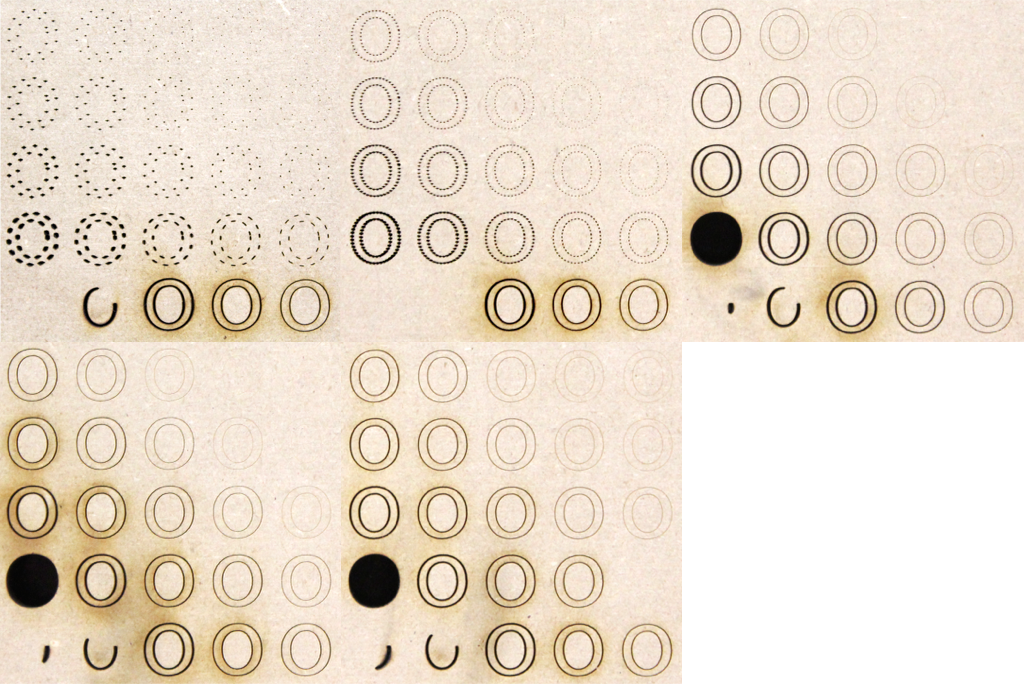
\includegraphics[width=0.4\textwidth]{figures/engravings}
  \caption{%
    The letter `O' engraved into a piece of particle board with a laser cutting machine.
    Each `O' is engraved with a different configuration.
    Each of the five cells was engraved with a different PPI (`pulse per inch')
    In each cell, the laser's speed grows along the x-axis, and power along the y-axis.
    If a user wants fine-grained control over appearance, they need to express these parameters with a slider-based interface.
  }\label{fig:engravings}
\end{figure}

We frequently use machines to tailor things to our subjective preferences.
We may begin our day by adjusting a dial on a toaster to cook it to the right crispness, and later adjust the brightness of an image in a photo-editing program using a slider.
Fabrication devices with complex mechanical operation are increasingly entering home and hobby spaces.
Having a set of `go-to' presets is unlikely to be helpful when experimenting with new materials and designs.
To achieve their subjective preferences in unfamiliar circumstances, users will need a way to quickly experiment with parameters.

Today's interfaces are not well-equipped to help users who are seeking to configure these machines for the first time.
One challenge is that users are reluctant to read documentation on how to use technologies.
It is well established that software users don't read detailed documentation~\cite{carroll_nurnberg_1990}.
Another problem is that these machines have unfamiliar conceptual models (see Norman's definition~\cite{norman_design_2002}).
It is hard for users to conceptualize the impact that parameters like laser power, speed, and ``PPI'' will have on a workpiece (see Figure~\ref{fig:engravings}).

This paper adapts two algorithms to help a user explore a parameter space to achieve their subjective preferences.
It reports on user perceptions of trustworthiness, randomness, and accuracy of the methods.
This is the first step in a systematic evaluation of algorithms for this problem. 
It focuses on the output of a laser cutter, a fabrication machine some scholars envision as being part of the home workshop of the future.

\if 0
To frame this problem in a way I could test it, I engraved this O with a bunch of different settings.
Then in a couple of interfaces, I showed people one of the Os as a goal, and a set of options that they had to rank.
For different ranking schemes, I change the front-end.
What are the pairs of algorithms and interfaces I use?

Consider what it takes to configure a laser cutter to engrave workpieces.
Consider the trivial ``O'' design in Figure~\ref{fig:rasters}.
Three parameters control the depth, speed, and resolution of the image etched into the material.
Improper values cause the image to appear only faintly, or scorch the material.
\fi

Both algorithms take \emph{comparisons} of configurations as input.
To justify this, I refer to a discussion from~\cite{brochu_tutorial_2010}.
Human evaluation of single choices can be unreliable due to drift and anchoring.
In addition, research in psychology~\cite{tversky_advances_1992} and economics~\cite{kingsley_preference_2006} has established human models of choice, and explored phenomena such as preference refinement.
This past work suggests humans are capable of producing good comparisons.
For future work, it provides a lens for evaluating the cost of providing comparison-based inputs to algorithms.

\if 0
Each configuration will comprise laser power, speed, frequency, and resolution.
The algorithm will suggest configurations and demonstrate them by rastering an image.
The algorithm will collect a user's rating of raster quality.
As the learned model will predict an continuous value, I will draw from past work for actively learning continuous-value models (e.g.~\cite{sugiyama_active_2008}).
\fi

\if 0
To understand the trade-offs of this method of mixed initiative parameter space exploration, I ran a usability study.
This was on Mechanical Turk with 28 participants.
They were asked to recover a configuration for rastering an image that matches an exemplar I provide.
The method of parameter exploration was varied between two algorithms: Nelder-Mead~\cite{nelder_simplex_1964} and an instantiation of Bayesian optimization~\cite{brochu_tutorial_2010}.
I measured the total number of configurations tested, and Likert scale feedback on perceptions of the algorithms.
I also report on a pilot study that compares how people work with a standard slider-based interface for parameter exploration vs.\ and interface based on Nelder-Mead optimization.
\fi
